\input{../../input/main}

\begin{document}

\begin{center}
  \Large{\textbf{Городской центр физического образования, 10 класс.}\\
  \textit{Серия 22, 9 апреля 2015.}}
\end{center}

\begin{center}
  \Large\textbf{ Окончание электростатики. }
\end{center}

\task{ Современный лабораторный блок питания работает так: сначала ему
  задаются значения тока $I_0$ и напряжения $U_0$. После подключения
  нагрузки блок сам выбирает один из двух режимов: либо поддерживает
  напряжение на нагрузке равным $U_0$, если при этом ток через
  нагрузку не больше $I_0$ --- либо поддерживает ток через нагрузку
  равным $I_0$, если при этом напряжение на нагрузке не больше
  $U_0$. В качестве нагрузки к такому блоку питания подсоединяют
  незаряженный конденсатор емкостью $C$. Нарисуйте график зависимости
  напряжения $U$ на нём от времени $t$.  }

\task{ Обкладками плоского конденсатора служат две параллельные
  квадратные металлические пластины со стороной $a$, расположенными на
  расстоянии $d$ ($d \ll a$). Между обкладками находится слюдяная
  пластинка толщиной $d/2$, размеры которой совпадают с размерами
  обкладок. Конденсатор подключен через резистор $R$ к источнику
  постоянного напряжения $U$. Слюдяную пластинку медленно с постоянной
  скоростью $V$ вытягивают из конденсатора. Какое количество теплоты
  выделится при этом на резисторе?  }

\taskpic{ Пластины плоского конденсатора имеют форму правильного
  треугольника, расстояние между пластинами много меньше их
  размеров. Внутри конденсатора, вдали от краев электрическое поле
  равно $E_0$. Чему равно поле в середине отрезка \textbf{AB},
  соединяющего ближайшие углы двух пластин конденсатора? Отрезок
  \textbf{AB} перпендикулярен плоскости пластин. Что будет, если
  пластины имеют форму правильного пятиугольника? Ответ обоснуйте. }
{
  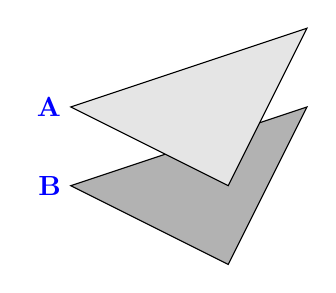
\begin{tikzpicture}
    \draw[fill=gray!60] (0,-1) node[left,blue] {\textbf{B}} -- (3,0) --
    (2,-2) -- cycle;
    \draw[fill=gray!20] (0,0) node[left,blue] {\textbf{A}} -- (3,1) --
    (2,-1) -- cycle;
  \end{tikzpicture}
}

\task{ Сложный конденсатор состоит из четырёх одинаковых пластин
  площадью $S=1 \mbox{ м}^{2}$ каждая, расположенных параллельно друг
  другу. Расстояние между средними пластинами $b$ и $c$ равно $l=2$
  см. Расстояние между пластинами $a$ и $b$, $c$ и $d$ равно
  $l_1=l/2$. Пластины бис подключены к идеальному источнику напряжения
  с $\mathcal{E}=120$ В через резистор $R_{1}$. В начальном состоянии
  ключ \textbf{K} разомкнут. 1) Нарисуйте эквивалентную схему сложного
  конденсатора после замыкания ключа \textbf{K} и найдите его ёмкость
  $C$. 2) Какое количество теплоты $Q$ выделится на резисторах $R_1$ и
  $R_2$ (в сумме) при замыкании ключа \textbf{K}?  Электрическая
  постоянная $\eps_0 = 8{,}85 \cdot 10^{-12}$ Ф/м. \textit{Указание.}
  Воспользуйтесь законом сохранения энергии. }
\begin{center}
  \begin{tikzpicture}[circuit ee IEC, thick]
    \draw[ultra thick] (0,0) -- ++(down:3cm) node[midway,left] {$a$};
    \draw[ultra thick] (1,0) -- ++(down:3cm) node[midway,right] {$b$};; 
    \draw[ultra thick] (3,0) -- ++(down:3cm) node[midway,left] {$c$};; 
    \draw[ultra thick] (4,0) -- ++(down:3cm) node[midway,right] {$d$};;
    \draw (3,0) -- ++(up:0.2cm) -- ++(right:0.5cm) -- ++(up:0.5cm)
    to[resistor={info'={$R_{1}$}}] ++(left:1.5cm)
    to[battery={info'={$\mathcal{E}$}}] ++(left:1.5cm) -- 
    ++(down:0.5cm) --++(right:0.5cm) -- ++(down:0.2cm);
    \draw (0,-3) -- ++(down:0.5cm) to[resistor={info'={$R_2$}}] ++(right:2cm)
    to[make contact={info'={\textbf{K}}}] ++(right:2cm) -- ++(up:0.5cm); 
  \end{tikzpicture}
\end{center}


\end{document}


%%% Local Variables: 
%%% mode: latex
%%% TeX-engine:xetex
%%% TeX-PDF-mode: t
%%% End:
